\subsection{Unified Image and Video Generative Architecture}
\label{sec:architecture}
% \dq{@Weijie, Tianqi, Zijian, Jianwei}

% In this section, we introduce the Transformer design in \nameofmethod{}. We adopt a unified Full Attention mechanism, primarily based on the following three reasons:
% Firstly, it has been validated to exhibit superior performance compared to divided spatiotemporal attention.
% Secondly, it supports unified generation for both images and videos, simplifying the training process while facilitating better model scalability.
% Lastly, it leverages existing LLM-related acceleration capabilities more effectively, enhancing both model training and inference efficiency.

% For a given video-text pair, the model is performed within the 3D latent space mentioned in section \ref{3dVAE}.  More specifically, for the video branch, the input is first compressed into latents of shape $T\times C \times H \times W$. We treat images as single-frame videos, to unify the input processing. These latents are then patchified and unfolded into a 1D sequence of tokens with a length of $\frac{T}{k_t}\cdot \frac{H}{k_h}\cdot \frac{W}{k_w}$, using a 3D convolution with a kernel size of $k_t\times k_h\times k_w$.  For the text branch, we first employ an advanced LLM to encode it into a text embedding sequence, which contains fine-grained semantics information. Meanwhile, we use the CLIP model to extract pooled text representation, which contains global information, which are added to the timestep embedding after dimensionality expansion.
\begin{figure}[ht]
    \centering
    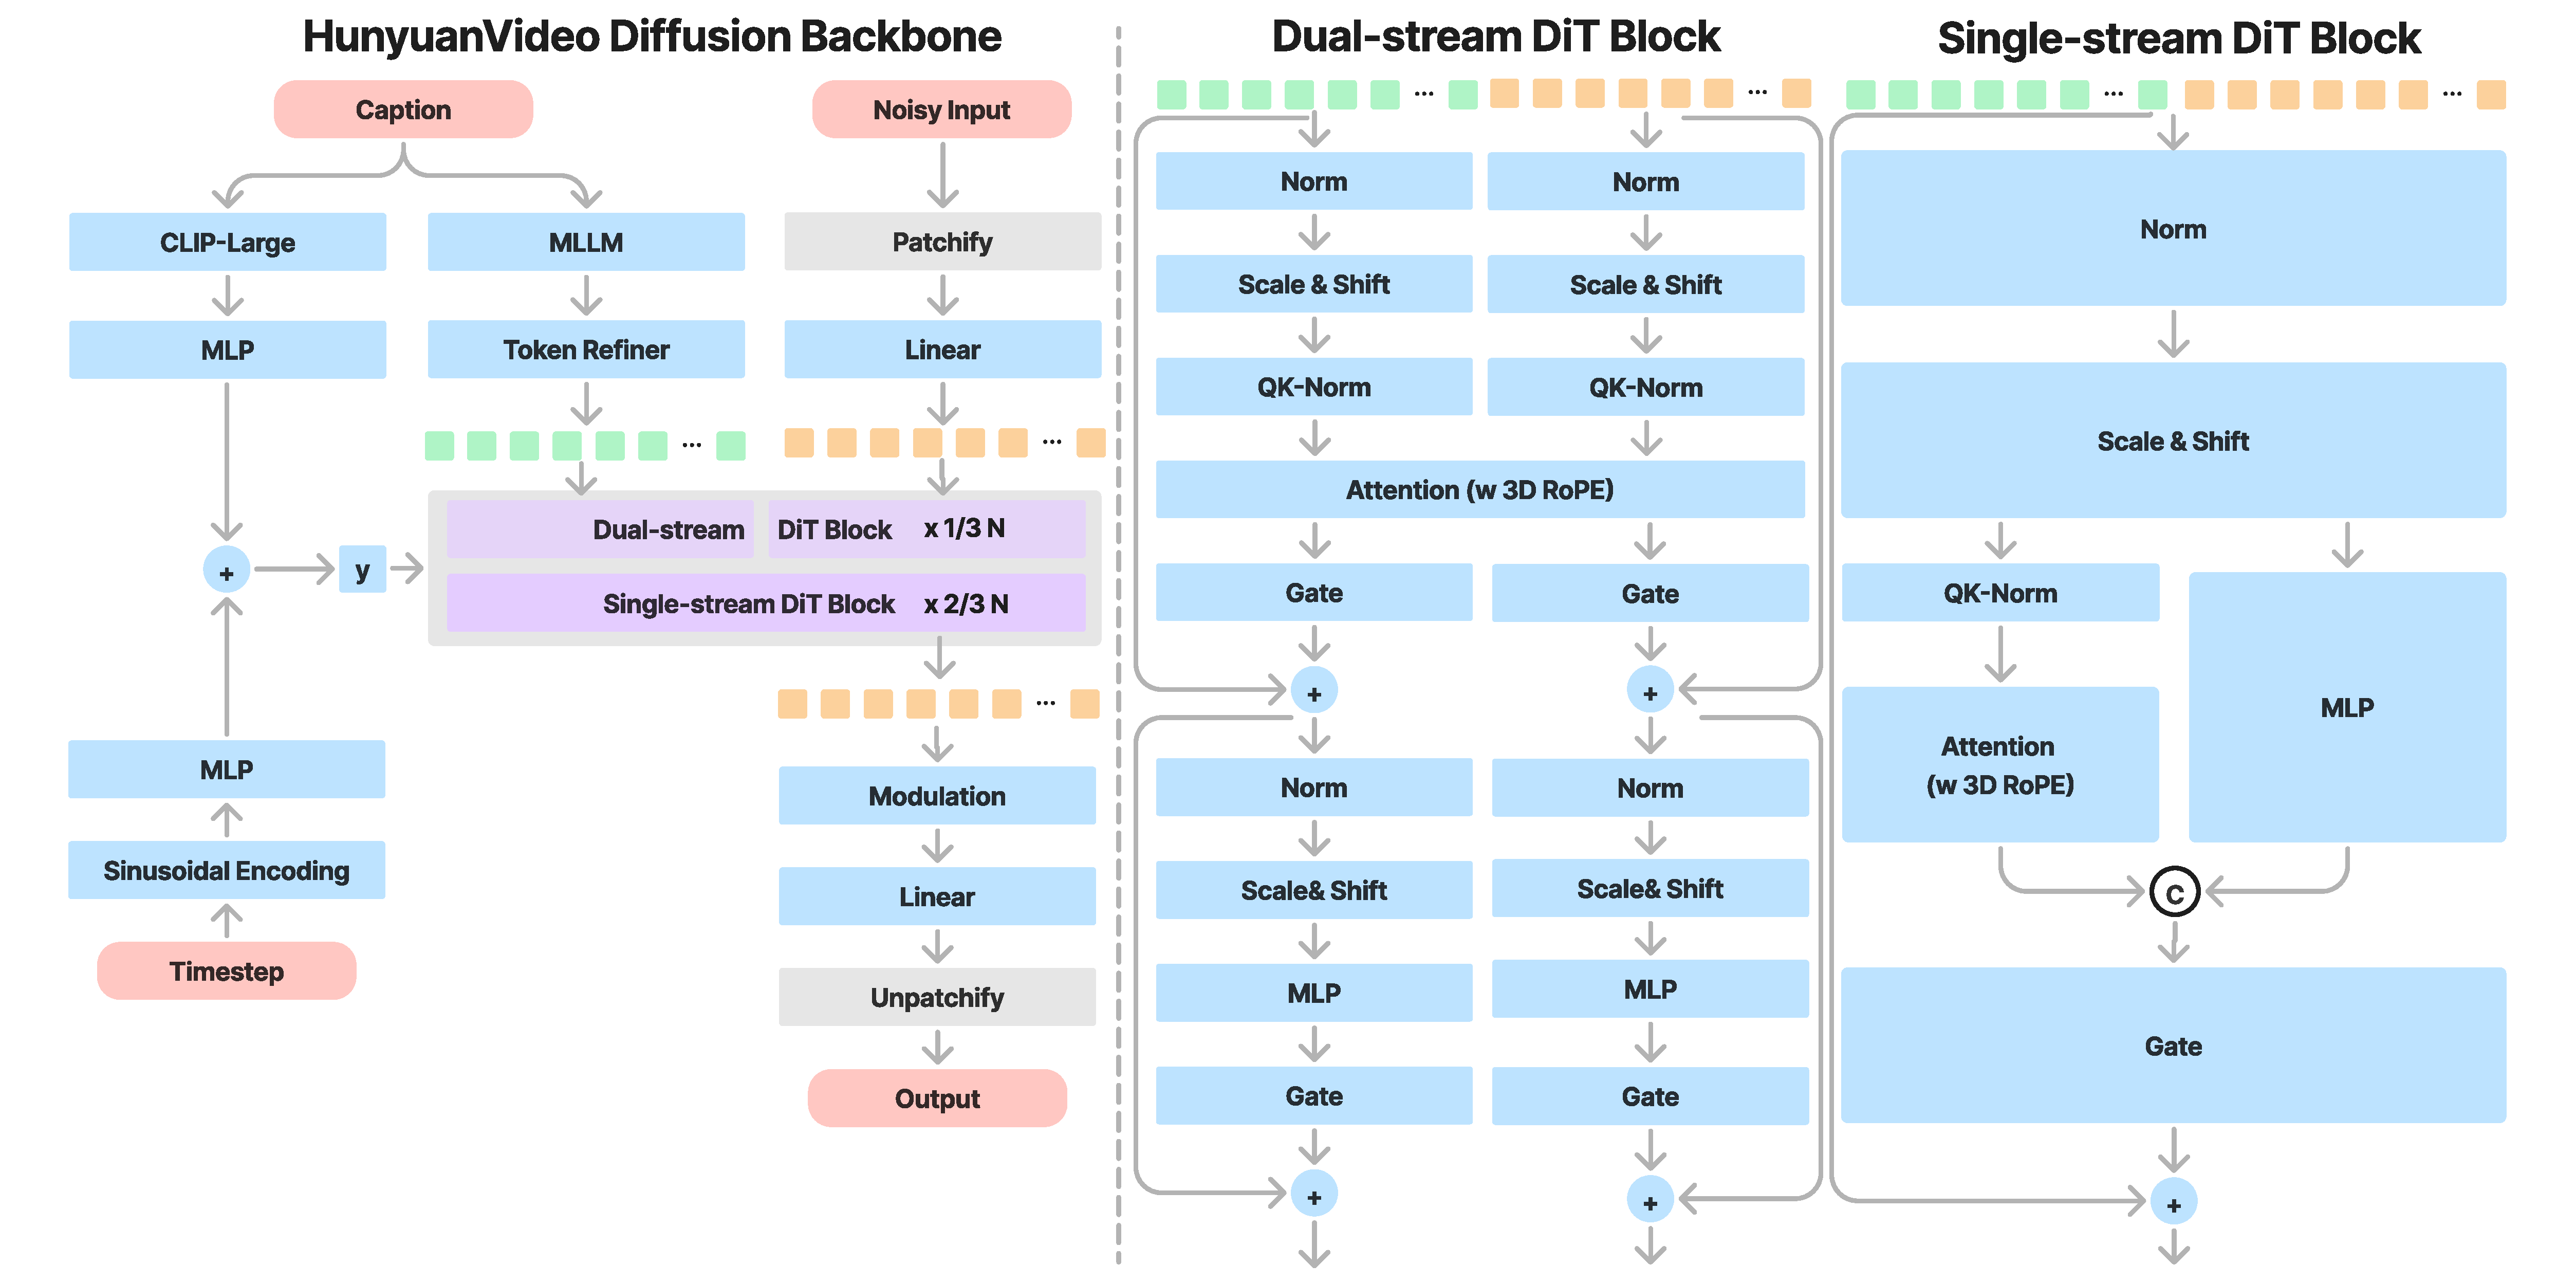
\includegraphics[width=\linewidth]{figures/dit_backbone.pdf}
    \caption{ The architecture of our \nameofmethod{} Diffusion Backbone.}
    \label{fig:dit_bnackbone}
\end{figure}

In this section, we introduce the Transformer design in \nameofmethod{}, which employs a unified Full Attention mechanism for three main reasons:
Firstly, it has demonstrated superior performance compared to divided spatiotemporal attention~\cite{videoworldsimulators2024,polyak2024movie,yang2024cogvideox,genmo2024mochi}.
Secondly, it supports unified generation for both images and videos, simplifying the training process and improving model scalability.
Lastly, it leverages existing LLM-related acceleration capabilities more effectively, enhancing both training and inference efficiency.
The model structure is illustrated in Figure \ref{fig:dit_bnackbone}.

\textbf{Inputs.} For a given video-text pair, the model operates within the 3D latent space described in Section \ref{3dVAE}. Specifically, for the video branch, the input is first compressed into latents of shape $T \times C \times H \times W$. To unify input processing, we treat images as single-frame videos. These latents are then patchified and unfolded into a 1D sequence of tokens with a length of $\frac{T}{k_t} \cdot \frac{H}{k_h} \cdot \frac{W}{k_w}$ using a 3D convolution with a kernel size of $k_t \times k_h \times k_w$. For the text branch, we first use an advanced LLM to encode the text into a sequence of embeddings that capture fine-grained semantic information. Concurrently, we employ the CLIP model to extract a pooled text representation containing global information. This representation is then expanded in dimensionality and added to the timestep embedding before being fed into the model.

\textbf{Model Design.}  To integrate textual and visual information effectively, we follow a similar strategy of "Dual-stream to Single-stream" hybrid model design as introduced in \cite{FLUX} for video generation. In the dual-stream phase, video and text tokens are processed independently through multiple Transformer blocks, enabling each modality to learn its own appropriate modulation mechanisms without interference. In the single-stream phase, we concatenate the video and text tokens and feed them into subsequent Transformer blocks for effective multimodal information fusion. This design captures complex interactions between visual and semantic information, enhancing overall model performance.

\textbf{Position Embedding.} To support multi-resolution, multi-aspect ratio, and varying duration generation, we use Rotary Position Embedding (RoPE)~\cite{su2023roformer} in each Transformer block. RoPE applies a rotary frequency matrix to the embeddings, enhancing the model's ability to capture both absolute and relative positional relationships, and demonstrating some extrapolation capability in LLMs. Given the added complexity of the temporal dimension in video data, we extend RoPE to three dimensions. Specifically, we compute the rotary frequency matrix separately for the coordinates of time ($T$), height ($H$), and width ($W$). We then partition the feature channels of the query and key into three segments $(d_t, d_h, d_w)$, multiply each segment by the corresponding coordinate frequencies and concatenate the segments. This process yields position-aware query and key embeddings, which are used for attention computation.

% This extension encodes spatial positions within each video frame and temporal positions across frames, improving the model's understanding and generation capabilities for video content.

For detailed model settings, please refer to Table~\ref{tab:model_settings}.
\begin{table}[t]
  \centering
  \footnotesize
  \caption{Architecture hyperparameters for the \nameofmethod{} 13B parameter foundation model.}
  \begin{tabular}{ccccccc}
  \toprule
  \textbf{\makecell{Dual-stream \\Blocks}} & \textbf{\makecell{Single-stream \\Blocks}} & \textbf{\makecell{Model \\Dimension}} & \textbf{\makecell{FFN \\Dimension}} & \textbf{\makecell{Attention \\Heads}} & \textbf{\makecell{Head dim}} & $(d_t, d_h, d_w)$	\\
  \midrule
  20 & 40 & 3072 & 12288 & 24 & 128 & (16, 56, 56) \\
  \bottomrule
  \end{tabular}%
  \label{tab:model_settings}
\end{table}

% This model architecture exhibits excellent performance and reduces computational complexity. Compared to fully single-stream models[][], visual and semantic tokens are processed separately in the dual-stream stage, resulting in fewer tokens and improved computational efficiency through parallel processing. Although more tokens need to be processed in the single-stream stage, the earlier stages have already extracted more refined features, thereby reducing the overall training complexity.

\subsection{Text encoder}
% \dq{@Zijian, Jianwei, Weijie, Tianqi}

In generation tasks like text-to-image and text-to-video, the text encoder plays a crucial role by providing guidance information in the latent space. Some representative works~\cite{podell2023sdxl, esser2024scaling, li2024hunyuandit} typically use pre-trained CLIP~\cite{radford2021learning} and T5-XXL~\cite{raffel2020exploring} as text encoders where CLIP uses Transformer Encoder and T5 uses an Encoder-Decoder structure. In contrast, we utilize a pre-trained Multimodal Large Language Model~(MLLM) with a Decoder-Only structure as our text encoder, which has following advantages: (i) Compared with T5, MLLM after visual instruction finetuning has better image-text alignment in the feature space, which alleviates the difficulty of instruction following in diffusion models; (ii) Compared with CLIP, MLLM has been demonstrated superior ability in image detail description and complex reasoning~\cite{liu2024visual}; (iii) MLLM can play as a zero-shot learner~\cite{brown2020language} by following system instructions prepended to user prompts, helping text features pay more attention to key information. In addition, as shown in Fig.~\ref{fig:text-encoder}, MLLM is based on causal attention while T5-XXL utilizes bidirectional attention that produces better text guidance for diffusion models. Therefore, we follow~\cite{ma2024exploring} to introduce an extra bidirectional token refiner for enhancing text features.
%
We have configured \nameofmethod{} with a series of MLLMs~\cite{sun2024hunyuanlargeopensourcemoemodel,2023xtuner,glm2024chatglm} for different purposes. Under each setting, MLLMs have shown superior performance over conventional text encoder.
% With extensive experiments, we have demonstrated the effectiveness of MLLM as the text encoder on smaller \nameofmethod{} by integrating various open-source MLLMs~\cite{sun2024hunyuanlargeopensourcemoemodel,2023xtuner,glm2024chatglm}.

In addition, CLIP text features are also valuable as the summary of the text information. As shown in Fig.~\ref{fig:dit_bnackbone} We adopt the final non-padded token of CLIP-Large text features as a global guidance, integrating into the dual-stream and single-stream DiT blocks. 

\begin{figure}[t]
    \centering
    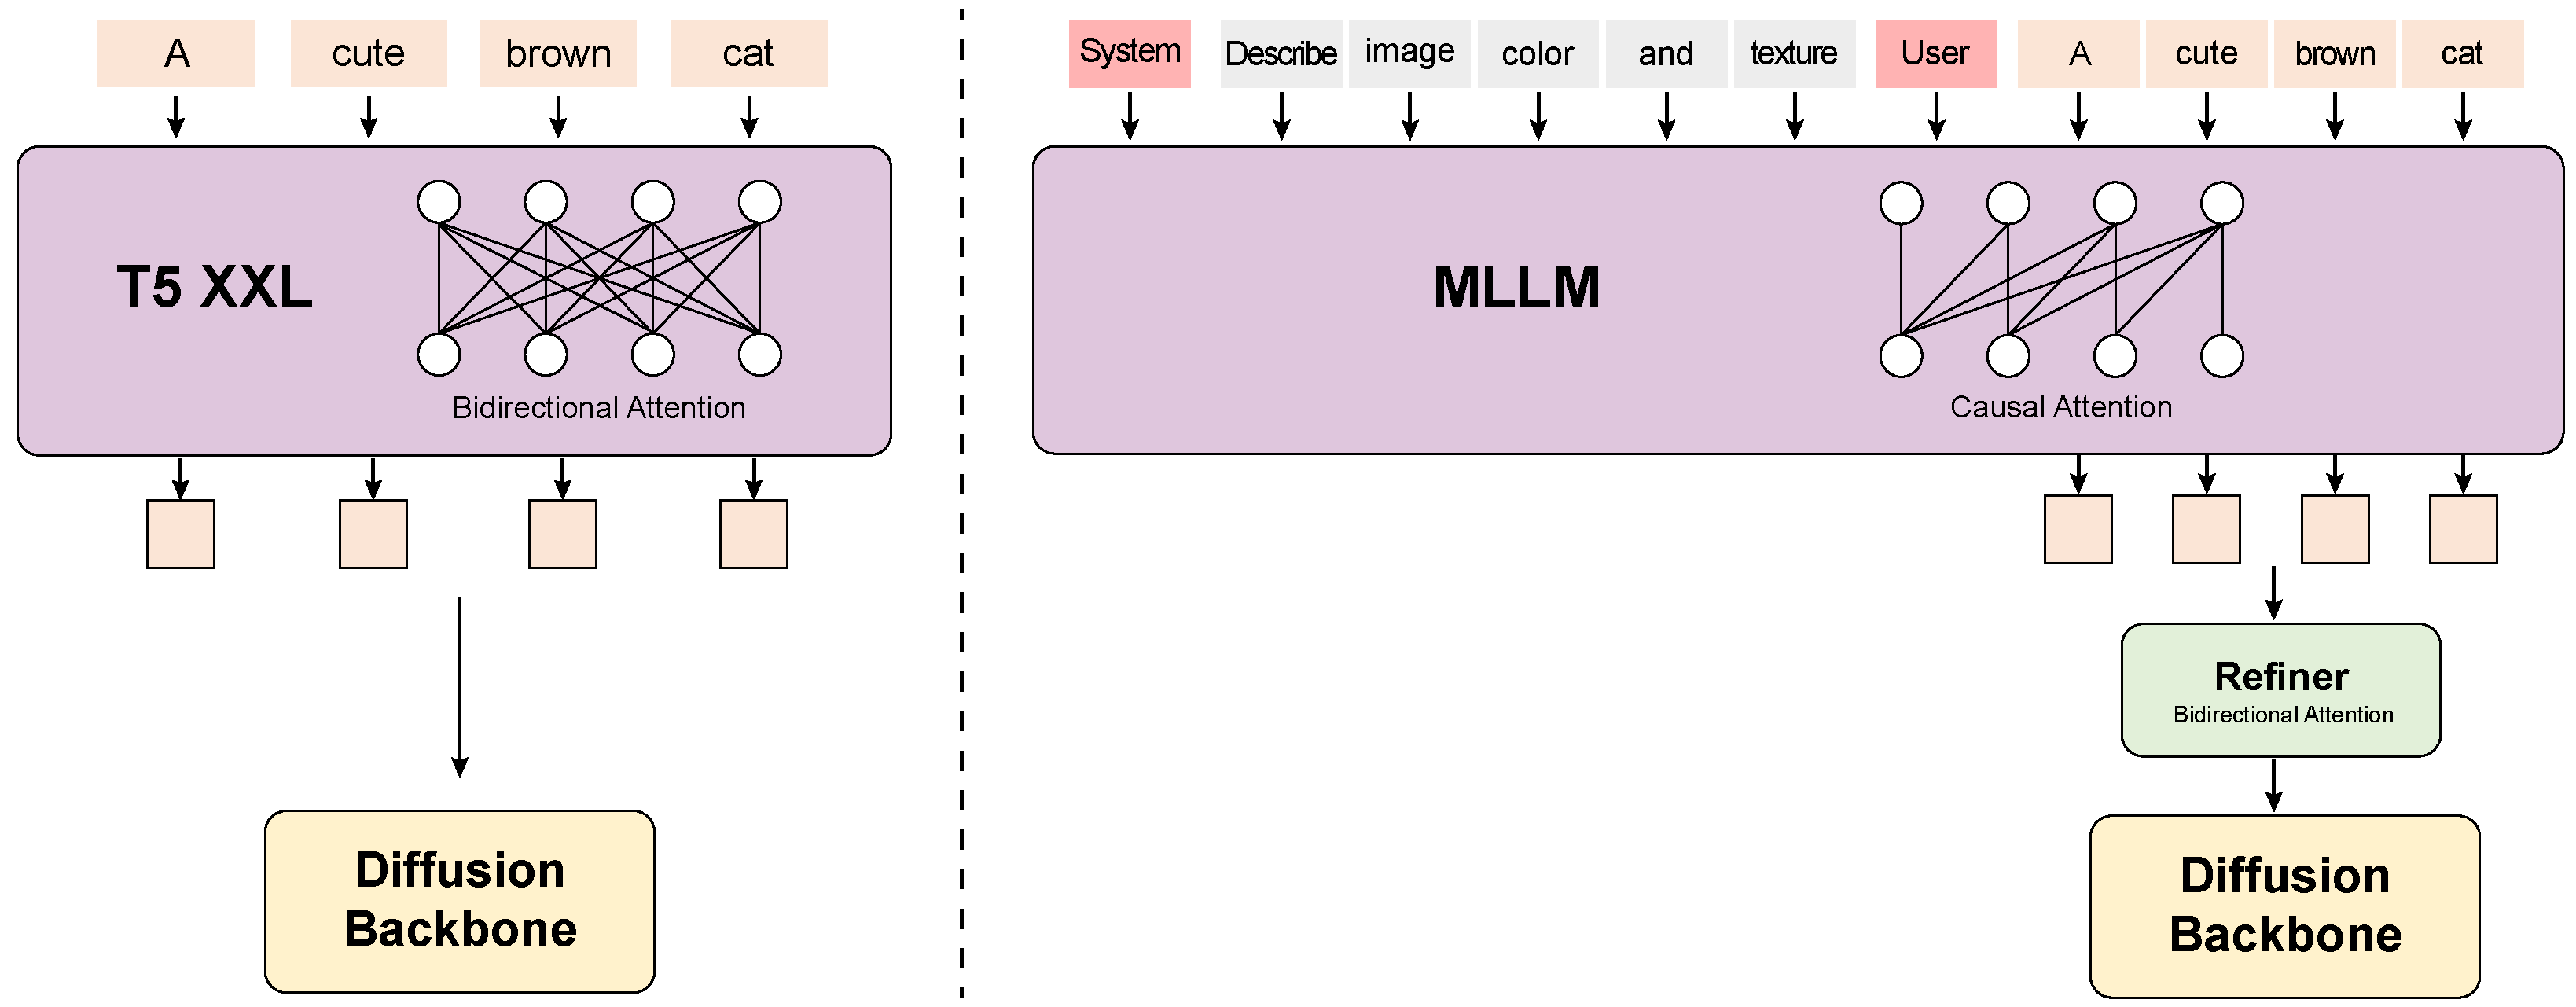
\includegraphics[width=0.9\linewidth]{figures/text_encoder_en.pdf}
    \caption{Text encoder comparison between T5 XXL and the instruction-guided MLLM introduced by \nameofmethod{}.}
    \label{fig:text-encoder}
\end{figure}


\subsection{Model Scaling}
Neural scaling laws~\cite{kaplan2020scaling,hoffmann2022training} in language model training offer a powerful tool for understanding and optimizing the performance of machine learning models. By elucidating the relationships between model size ($N$), dataset size ($D$), and computational resources ($C$), these laws help drive the development of more effective and efficient models, ultimately advancing the success of large model training.

\begin{figure}[t]
    \centering
    \begin{subfigure}{0.325\textwidth}
        \centering
        \includegraphics[width=\textwidth]{figures/scaling_law.pdf}
        \caption{T2X(I) Loss curve and envelope}
        \label{fig:scaling-laws}
    \end{subfigure}
    \hfill
    \begin{subfigure}{0.325\textwidth}
        \centering
        \includegraphics[width=\textwidth]{figures/computation_vs_parameter.pdf}
        \caption{T2X(I) Power law of $C$ and $N$}
        \label{fig:computation-vs-parameter}
    \end{subfigure}
    \hfill
    \begin{subfigure}{0.325\textwidth}
        \centering
        \includegraphics[width=\textwidth]{figures/computation_vs_token.pdf}
        \caption{T2X(I) Power law of $C$ and $D$}
        \label{fig:computation-vs-token}
    \end{subfigure}
    \hfill
    \begin{subfigure}{0.325\textwidth}
        \centering
        \includegraphics[width=\textwidth]{figures/video_scaling_law.pdf}
        \caption{T2X(V) Loss curve and envelope}
        \label{fig:video-scaling-laws}
    \end{subfigure}
    \hfill
    \begin{subfigure}{0.325\textwidth}
        \centering
        \includegraphics[width=\textwidth]{figures/video_computation_vs_parameter.pdf}
        \caption{T2X(V) Power law of $C$ and $N$}
        \label{fig:video-computation-vs-parameter}
    \end{subfigure}
    \hfill
    \begin{subfigure}{0.325\textwidth}
        \centering
        \includegraphics[width=\textwidth]{figures/video_computation_vs_token.pdf}
        \caption{T2X(V) Power law of $C$ and $D$}
        \label{fig:video-computation-vs-token}
    \end{subfigure}
    \caption{Scaling laws of DiT-T2X model family. On the top-left (a) we show the loss curves of the T2X(I) model on a log-log scale for a range of model sizes from 92M to 6.6B. We follow~\cite{hoffmann2022training} to plot the envelope in gray points, which are used to estimate the power-law coefficients of the amount of computation ($C$) vs model parameters ($N$) (b) and the computation vs tokens ($D$) (c). Based on the scaling law of the T2X(I) model, we plot the scaling law of the corresponding T2X(V) model in (d), (e), and (f).}
    \label{fig:image_scaling_laws}
\end{figure}

In contrast to prior scaling laws on large language models~\cite{kaplan2020scaling,hoffmann2022training,touvron2023llama,achiam2023gpt,anil2023palm} and image generation models~\cite{li2024scalability,kilian2024computational}, video generation models typically rely on pre-trained image models. Consequently, our initial step involved establishing the foundational scaling laws pertinent to text-to-image. Building upon these foundational scaling laws, we subsequently derived the scaling laws applicable to the text-to-video model. By integrating these two sets of scaling laws, we were able to systematically determine the appropriate model and data configuration for video generation tasks. 

% Specifically, we developed a series of models with sizes ranging from 92M to 6.6B. Each model was trained on up to 500 billion tokens, using consistent hyperparameters and the same dataset with 256p resolution. By examining the final loss of these models, we refer to \cite{hoffmann2022training} to establish the relationship between training FLOPs $C$ and model parameters $N$ as $ N = a\cdot C^{b}$, where $a$ and $b$ denotes the coefficient to be fitted.

\subsubsection{Image model scaling law}
% \dq{@Zijian, Jianwei}

Kaplan et.al~\cite{kaplan2020scaling} and Hoffmann et.al~\cite{hoffmann2022training} explored emperical scaling laws for language models on cross-entropy loss. In the field of diffusion based visual generation, Li et.al~\cite{li2024scalability} study the scaling properties on UNet, while transformer based works such as DiT~\cite{peebles2023scalable}, U-ViT~\cite{bao2023all}, Lumina-T2X~\cite{gao2024lumina}, and SD3~\cite{esser2024scaling} only study the scaling behavior between sample quality and network complexity, leaving the power-laws about the computation resources and MSE loss used by diffusion models unexplored.

In order to fill the gap, we develop a family of DiT-like models, named as DiT-T2X to distinguish from the original DiT, where X can be the image (I) or the video (V).
DiT-T2X applies T5-XXL~\cite{raffel2020exploring} as the text encoder and the aformentioned 3D VAE as the image encoder. The text information is injected to the model according to cross-attention layers. The DiT-T2X family has seven sizes ranging from 92M to 6.6B. The models were trained using DDPM~\cite{ho2020denoising} and v-prediction~\cite{salimans2022progressive} with consistent hyperparameters and the same dataset with 256px resolution. We follow the experiment method introduced by~\cite{hoffmann2022training} and build the neural scaling laws to fit 
\begin{equation}\label{eq:scaling_law}
N_{opt}=a_1C^{b_1},\quad D_{opt}=a_2C^{b_2}.    
\end{equation}

As shown in Fig.~\ref{fig:image_scaling_laws} (a), the loss curve of each model decreases from top left to bottom right, and it always passes through the loss curve of the larger size model adjacent to it. It means that each curve will form two intersections with curves of the larger and the smaller models. Under the corresponding computation resources between the two intersections, the middle-sized model is optimal (with the lowest loss). After obtaining the envelope of lowest losses across all the x-axis values, we fill the Equation ~\eqref{eq:scaling_law} to find out that $a_1=5.48\times10^{-4}, b_1=0.5634, a_2=0.324$ and $b_2=0.4325$, where the units of $a_1, a_2, N_{opt}, D_{opt}$ are billions while $C$ has a unit of Peta FLOPs. The Fig.~\ref{fig:image_scaling_laws} (b) and Fig.~\ref{fig:image_scaling_laws} (c) show that DiT-T2X(I) family fits the power law quite well. Finally, given computation budgets, we can calculate the optimal model size and dataset size. 

\subsubsection{Video model scaling law}
Based on the scaling law of the T2X(I) model, we select the optimal image checkpoint (\textit{i.e.,} the model on the envelope) corresponding to each size model to serve as the initialization model for the video scaling law experiment. Fig.~\ref{fig:image_scaling_laws} (d), Fig.~\ref{fig:image_scaling_laws} (e), and Fig.~\ref{fig:image_scaling_laws} (f) illustrate the scaling law results of the T2X(V) model, where $a_1=0.0189, b_1=0.3618, a_2=0.0108$ and $b_2=0.6289$.
Based on the results of Fig.~\ref{fig:image_scaling_laws} (b) and Fig.~\ref{fig:image_scaling_laws} (e), and taking into account the training consumption and inference cost, we finally set the model size to 13B. Then the number of tokens for image and video training can be calculated as shown in Fig.~\ref{fig:image_scaling_laws} (c) and Fig.~\ref{fig:image_scaling_laws} (f). It is worth noting that the amount of training tokens calculated by image and video scaling laws is only related to the first stage of training for images and videos respectively. The scaling property of progressive training from low-resolution to high-resolution will be left explored in future work.

% \dq{@Tianqi, Weijie}



